\begin{frame}{Other activities}
    \begin{itemize}
        \item Synthetic Eddy Method \href{https://www.theoj.org/joss-papers/joss.05565/10.21105.joss.05565.pdf}{publication}
        \item JuliaCon 2023 conference
        \item Co-author AIAA 2023 conference paper
    \end{itemize}
    
    \begin{itemize}
        \item Testing standard passive flow controls (no improvement in aerodynamic efficiency)
    \end{itemize}
    \begin{figure}[h]
        \centering          
        \begin{subfigure}[h]{0.30\textwidth}
                 \centering
            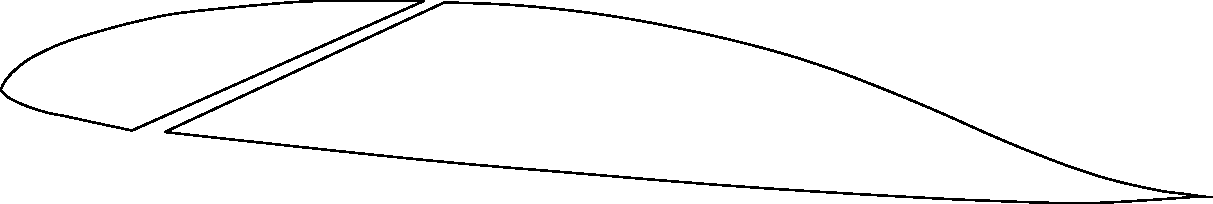
\includegraphics[width=\textwidth]{Slot.pdf}
            \caption{Slot}
       \end{subfigure}
       \hfill	
       \begin{subfigure}[h]{0.30\textwidth}
                \centering
           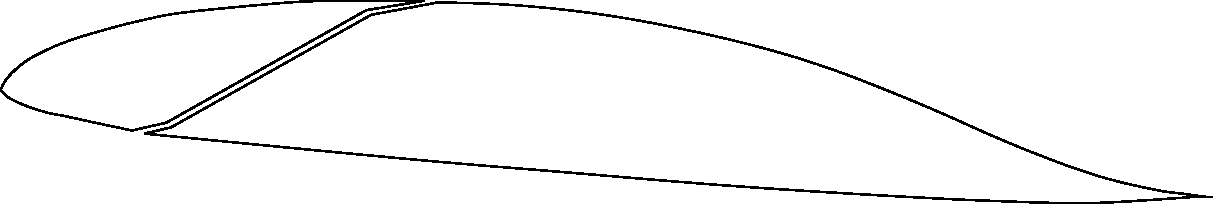
\includegraphics[width=\textwidth]{Slot-curved.pdf}
           \caption{Slot curved}
        \end{subfigure}
             \hfill
        \begin{subfigure}[h]{0.30\textwidth}
         \centering
            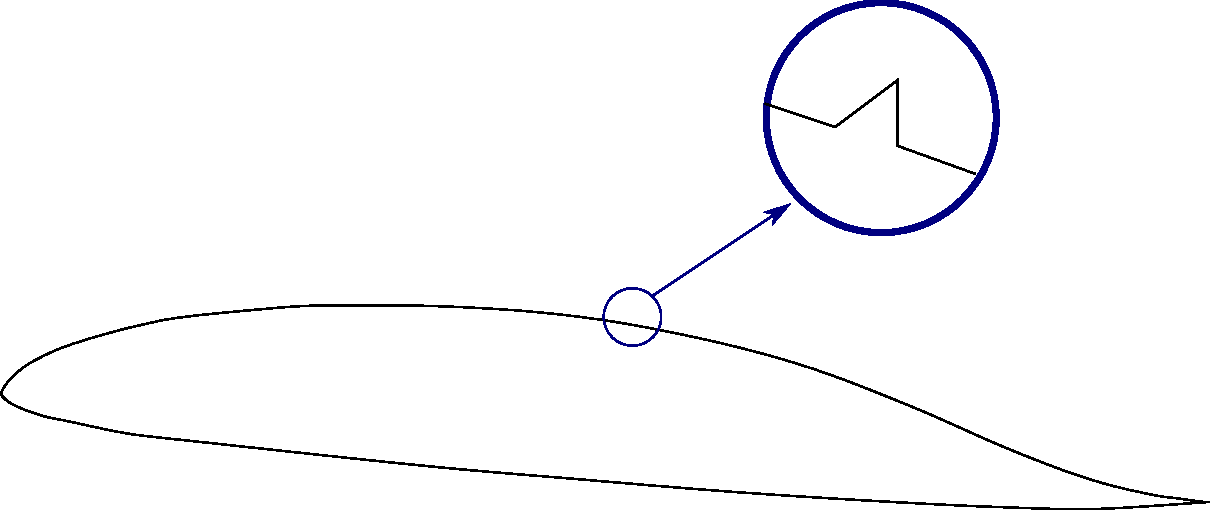
\includegraphics[width=\textwidth]{Riblet.pdf}
            \caption{Riblet}
        \end{subfigure}
        \caption{Passive Flow Controls}
        \end{figure} 
    \end{frame}
    
    
    
    \begin{frame}{Elements of novelty}
    \begin{itemize}
        \item Systematic usage of Julia in fluid-dynamics
        \item Usage of VMS for high Reynolds airfoil
        \item First LES code in Julia - fully parallelized - working with 3D airfoils up to Re $\num{500000}$ 
        \item Synthetic Eddy Method coded in Julia and coupled with the VMS
    \end{itemize}
    
    It has been challenging, but it seems we are on the right path!
    
    \end{frame}
    
    \begin{frame}{Next steps}
    Expected papers:
    \begin{itemize}
        \item VMS paper (prof. Janssens reading)
        \item Experimental validation of the LS-VMS - publish paper
        \item LC-VMS - (publish paper?)
    \end{itemize}
    
    Expected conferences:
    \begin{itemize}
        \item AIAA2024 conferences (LS-VMS, LC-VMS)
        \item DLES14 (VMS usage, validation test cases)
        \item ICAS2024 (Passive Flow Controls)
    \end{itemize}
    
    
    Expected research:
    \begin{itemize}
        \item Uncertainty Quantification using Polynomials Chaos Transformation on $\gamma-Re_\theta$ and VMS
        \item Start coding the adjoint optimization
        \item Test a passive flow control with the VMS
    \end{itemize}
    
    \end{frame}
    
    